\chapter{随机变量生成}
\section{方法介绍}
\subsection{反变换法}
\begin{newprop}[反变换法(Inverse-Transform)]
    \begin{itemize}
        \item 基本思想
        \begin{itemize}
            \item 已知:$F(x) \in[0,1],\ R\sim U[0,1] $
            \item 令$R=F(x)$,可以反解出$x = F^{-1}(R)$,如果反解出的$x$服从所需的分布,则问题的解。
        \end{itemize}
        \item 需要证明
        \begin{itemize}
            \item $F(x)$服从\textcolor{thid1}{均匀分布},即$F(x)\sim U[0,1]$
            \item 算出数据的CDF为所需的$F(x)$,即$P\left\lbrace F^{-1}(R)<x \right\rbrace = F(x) $
        \end{itemize}
    \end{itemize}
\end{newprop}
\begin{example}
    1.某分布的累积分布函数为:
    
    \begin{wrapfigure}[10]{r}{0.40\textwidth}
        \vspace*{-40pt}
        \begin{tikzpicture}[scale=1.3]
            \draw[-Stealth](-1,0)--(0,0)node[below]{$O$}--(3,0)node[below]{$x$};
            \draw[-Stealth](0,-1)--(0,2.5)node[left]{$y$};
            \foreach \x in{0,0.5,...,3}
            {
                \draw(\x,0)--(\x,0.05);
            }
            \foreach \x in{0,0.5,...,2}
            {
                \draw(0,\x)--(0.05,\x);
            }	
            \draw[domain=0:0.25,color=red]plot(\x,{2*\x});
            \draw[domain=0.25:2,color=red]plot(\x,{2*(3*\x+1)/7});
            \draw[domain=2:3,color=red]plot(\x,{2*1});
        \end{tikzpicture}
    \end{wrapfigure}
    $
    F(x)=
    \left\{  
    \begin{array}{lr} 
        0, & x\leqslant 0 \\ 
        x, & 0\leqslant x<  \frac{1}{4}\\ 
        \dfrac{3x+1}{7}, & \frac{1}{4}\leqslant x< 2  \\
        1, &x\geqslant 2
    \end{array}  
    \right.  
    $
    
    求出$F(x)$的逆函数
    
    $
    x = F^{-1}(r) = \left\{  
    \begin{array}{lr} 
        r, & 0\leqslant r < \frac{1}{4}\\
        \dfrac{7r-1}{3}, & \frac{1}{4} \leqslant r \leqslant 1
    \end{array}  
    \right. 
    $
\end{example}
\begin{example}
    2.\textcolor{thid2}{三角分布}:
    
    \begin{wrapfigure}[8]{r}{16em} % 纵向8行,图片靠右,宽度12.5em
        \vspace*{-36pt}
        \begin{tikzpicture}[scale = 1.2]
            \draw[-Stealth](-1,0)--(0,0)node[below left]{$O$}--(4,0)node[below]{$x$};
            \draw[-Stealth](0,-1)--(0,2.3)node[left]{$y$};
            \draw[thick,domain=0.5:1.5]plot(\x,{2*(\x-0.5)/(1.5-0.5)/(3-1.5)})node[above]{$y=f(x)$};;
            \draw[thick,domain=1.5:3]plot(\x,{2*(3-\x)/(3-1.5)/(3-1.5)});
            \draw[densely dashed](1.5,1.33)--(1.5,0)node[below]{$b$}
            (1.5,1.33)--(0,1.33)node[left]{$\frac{2}{c-a}$};
            \node(a)[below]at(0.5,0){$a$};
            \node(c)[below]at(3,0){$c$};
        \end{tikzpicture}
    \end{wrapfigure}
    
    概率密度函数:
    
    $
    f(x)=
    \left\{  
    \begin{array}{lr}  
        \dfrac{2(x-a)}{(b-a)(c-a)}, &a\leqslant x \leqslant b\\
        \dfrac{2(c-x)}{(c-b)(c-a)}, & b < x \leqslant c\\
        0, & elsewhere	    
    \end{array}  
    \right.
    $
    
    累积分布函数:
    
    $
    F(x)=
    \left\{  
    \begin{array}{lr}  
        0, & x\leqslant a\\
        \dfrac{(x-a)^{2}}{(b-a)(c-a)}, & a\leqslant x <b \\
        \dfrac{-x^{2}+2cx+ab-ac-bc}{(c-a)(c-b)}, & b\leqslant x <c\\
        1, & c \leqslant x
    \end{array}  
    \right.
    $
    
    逆函数:
    
    $
    F^{-1}(r)=
    \left\{  
    \begin{array}{lr}  
        \sqrt{(b-a)(c-a)r}+a, & 0\leqslant r <\dfrac{b-a}{c-a}\\
        c-\sqrt{(c-a)(c-b)(1-r)}, & \dfrac{b-a}{c-a} \leqslant r \leqslant 1
    \end{array}  
    \right.
    $
\end{example}
\begin{example}
    3.\textcolor{thid2}{均匀分布}:
    
    \begin{wrapfigure}[3]{r}{0.5\textwidth}
        \begin{tikzpicture}
            \centering
            \draw[-Stealth](-1,0)--(0,0)--(5,0)node[below]{$x$};
            \draw[-Stealth](0,-1)--(0,2.5)node[left]{$y$};
            \draw[domain=1:4]plot(\x,1.5);
            \draw[densely dashed](1,1.5)--(1,0)node[below]{$a$}
            (4,1.5)--(4,0)node[below]{$b$}
            (1,1.5)--(0,1.5)node[left]{$ \frac{1}{b-a} $};
        \end{tikzpicture}
    \end{wrapfigure}
    
    概率密度函数:
    
    $
    f(x)=
    \left\{  
    \begin{array}{lr}  
        \dfrac{1}{b-a}, &a<x<b\\
        0, & others	    
    \end{array}  
    \right.  
    $
    
    累积分布函数:
    
    $
    F(x)=
    \left\{  
    \begin{array}{lr} 
        0, & x<a \\ 
        \dfrac{x-a}{b-a}, & a \leqslant x \leqslant b \\
        0, & others	    
    \end{array}  
    \right.  
    $
    
    逆函数:
    
    $
    F^{-1}(r)= a+(b-a)r
    $
\end{example}
\begin{example}
    4.\textcolor{thid2}{指数分布}:
    
    \begin{wrapfigure}[10]{r}{0.40\textwidth}
        \vspace*{-70pt}
        \begin{tikzpicture}[scale=1.3]
            \draw[-Stealth](-1,0)--(0,0)node[below]{$O$}--(4,0)node[below]{$x$};
            \draw[-Stealth](0,-1)--(0,2.5)node[left]{$y$};
            \foreach \x in{0,0.5,...,3}
            {
                \draw(\x,0)--(\x,0.05);
            }
            \foreach \x in{0,0.5,...,2}
            `		{
                \draw(0,\x)--(0.05,\x);
            }	
            \draw[domain=0:3,color=cyan]plot(\x,{0.5*exp(-0.5*\x)});
            \draw[domain=0:3,color=blue]plot(\x,{exp(-\x)});
            \draw[domain=0:3,color=thid2]plot(\x,{1.5*exp(-1.5*\x)});
            \draw[domain=0:3,color=violet]plot(\x,{2*exp(-2*\x)});
            \draw[-Stealth](0.5,3)node{\footnotesize{$\lambda=2$}}--(0,2);
            \draw[-Stealth](1,2.5)node{\footnotesize{$\lambda=1.5$}}--(0,1.5);
            \draw[-Stealth](1.5,1.5)node{\footnotesize{$\lambda=1$}}--(0,1.0);
            \draw[-Stealth](2.5,0.5)node{\footnotesize{$\lambda=0.5$}}--(0,0.5);
        \end{tikzpicture}
    \end{wrapfigure}
    $
    f(x)=
    \left\{  
    \begin{array}{lr}  
        \lambda e^{-\lambda x}, &x>0\\
        0, & x \leqslant 0	    
    \end{array}  
    \right.  
    $
    
    累积分布函数为:
    
    $
    F(x)=
    \left\{  
    \begin{array}{lr} 
        0, & x\leqslant 0 \\ 
        1-e^{-\lambda x}, & x>0    
    \end{array}  
    \right.  
    $
    
    逆函数:
    
    $
    F^{-1}(r)= -\dfrac{\ln(1-r)}{\lambda}
    $
\end{example}
\begin{example}
    5.\textcolor{thid2}{威布尔分布}:
    
    \begin{wrapfigure}[3]{r}{0.48\textwidth}
        \vspace*{-32pt}
        \begin{tikzpicture}[scale=1]
            \draw[-Stealth](-1,0)--(0,0)node[below]{$O$}--(4,0)node[below]{$x$};
            \draw[-Stealth](0,-1)--(0,4)node[left]{$y$};
            \draw[domain=0:1,color=cyan]plot(\x,{3*4*(\x)^(4-1)*exp(-(\x)^4)});
            \draw[domain=1:4,color=cyan]plot(\x,{3*4*(\x)^(4-1)*exp(-(\x)^4)});
            \draw[domain=0:4,color=blue]plot(\x,{3*2*(\x)^(2-1)*exp(-(\x)^2)});
            \draw[domain=0:4,color=thid2]plot(\x,{3*exp(-(\x)^1)});
            \draw[domain=0.08:4,color=violet]plot(\x,{3*0.5*(\x)^(0.5-1)*exp(-(\x)^0.5)});
            \draw[-Stealth](-1,1)node{\footnotesize{$\beta=1$}}--(0.40,1.40);
            \draw[-Stealth](-1,2.5)node{\footnotesize{$\beta=1$}}--(0,3);
            \draw[-Stealth](2.3,2.8)node{\footnotesize{$\beta=2$}}--(0.75,2.56);
            \draw[-Stealth](2.7,3.5)node{\footnotesize{$\beta=4$}}--(1.08,3.6);
            \node at (2,-0.5){\footnotesize{$v=0, \alpha=1$}};
        \end{tikzpicture}
    \end{wrapfigure}
    随机变量$X$具有概率密度函数为:
    
    $
    f(x)=
    \left\{  
    \begin{array}{lr} 
        \dfrac{\beta}{\alpha}\left( \dfrac{x-v}{\alpha} \right)^{\beta-1}e^{-( \dfrac{x-v}{\alpha})^{\beta}} , &x \geqslant v  \\ 
        0, & x<v    
    \end{array}  
    \right.  
    $
    
    则称$X$服从参数为$c,\alpha, \beta$的\textcolor{thid2}{威布尔分布}$(\alpha>0, \beta>0)$
    
    其累积分布函数:
    
    $
    F(x)=
    \left\{  
    \begin{array}{lr} 
        1-e^{-(\dfrac{x-v}{\alpha})^{\beta}} , &x \geqslant v  \\ 
        0, & x<v    
    \end{array}  
    \right.  
    $
    
    逆函数:
    
    $
    F^{-1}(r)= \alpha \left[ -\ln(1-r) \right]^{1/\beta} \ (v = 0)
    $
\end{example}
\begin{example}
    6.\textcolor{thid2}{已知样本点序列}\textcolor{thid1}{的连续经验分布函数}
    \begin{itemize}
        \item 假设随机变量在相邻样本点之间\textcolor{thid1}{均匀分布}
        \item 假设随机变量在\textcolor{thid1}{各个区间的概率相同},都为\textcolor{thid1}{1/n}
        
        概率密度函数:
        $
        f(x)=
        \left\{  
        \begin{array}{lr} 
            \dfrac{1}{n(x_{i}-x_{i-1})}  , &x_{i-1}\leqslant x \leqslant x_{i},\ i = 1,2,\cdots,n\\
            0, &others
        \end{array}  
        \right.  
        $
        
        累积分布函数:$
        F(x)=
        \left\{  
        \begin{array}{lr} 
            0, & x<x_{0}\\
            \dfrac{n-1}{n} + \dfrac{x-x_{i-1}}{n(x_{i}-x_{i-1})}  , &x_{i-1}\leqslant x \leqslant x_{i},\ i = 1,2,\cdots,n\\
            1, &x>x_{n}
        \end{array}  
        \right.  
        $
        \begin{table}[H]
            \centering
            \begin{tabular}{lll}
                \arrayrulecolor{red}
                $R = \dfrac{x-x_{i-1}}{n(x_{i}-x_{i-1})}+\dfrac{i-1}{R}$ &
                &
                $x_{i-1}\leqslant x \leqslant x_{i},\ i = 1,2,\cdots,n$ \\ \hline
                \multicolumn{1}{|l}{$x = x_{i-1}+n\left( x_{i}-x_{i-1} \right) \left( R-\dfrac{i-1}{n} \right) $} &
                &
                \multicolumn{1}{l|}{$\dfrac{i-1}{n} \leqslant R \leqslant \dfrac{i}{n},\ i = 1,2,\cdots,n$} \\ \hline
            \end{tabular}
        \end{table}
    \end{itemize}
\end{example}
\begin{example}
    7.\textcolor{thid2}{已知样本频率}\textcolor{thid1}{的连续经验分布函数}
    \begin{itemize}
        \item 不同的区间具有不同的\textcolor{thid1}{概率密度}
        \item 概率密度函数为分段函数
        
        概率密度函数:
        $
        f(x)=
        \left\{  
        \begin{array}{lr} 
            \dfrac{p_{i}}{x_{i}-x_{i-1}} =\dfrac{c_{i}-c_{i-1}}{x_{i}-x_{i-1}}   , &x_{i-1}\leqslant x \leqslant x_{i},\ i = 1,2,\cdots,n\\
            0, &others
        \end{array}  
        \right.  
        $
        
        累积分布函数:$
        F(x)=
        \left\{  
        \begin{array}{lr} 
            0, & x<x_{0}\\
            c_{i-1} + \dfrac{c_{i}-c_{i-1}}{x_{i}-x_{i-1}}(x-x_{i-1})  , &x_{i-1}\leqslant x \leqslant x_{i},\ i = 1,2,\cdots,n\\
            1, &x>x_{n}
        \end{array}  
        \right.  
        $
        \begin{table}[H]
            \centering
            \begin{tabular}{lll}
                \arrayrulecolor{red}
                $R = c_{i-1} + \dfrac{c_{i}-c_{i-1}}{x_{i}-x_{i-1}}(x-x_{i-1}) $                  &  & $x_{i-1}\leqslant x \leqslant x_{i},\ i = 1,2,\cdots,n$                       \\ \hline
                \multicolumn{1}{|l}{$x = x_{i-1}+a_{i} \left( R-c_{i-1} \right) $}                &  & \multicolumn{1}{l|}{$c_{i-1} \leqslant R \leqslant c_{i},\ i = 1,2,\cdots,n$} \\ \hline
                $ a_{i} = \dfrac{x_{i}-x_{i-1}}{c_{i}-c_{i-1}} $ &  &                                                                              
            \end{tabular}
        \end{table}
    \end{itemize}
\end{example}

\begin{wraptable}{r}{1.2cm}
    
    \centering
    \begin{tabular}{cc}
        \hline
        区间            & 频率 \\ \hline
        $15\sim 30$   & 10 \\
        $30\sim 45$   & 20 \\
        $45\sim 60$   & 25 \\
        $60\sim 90$   & 35 \\
        $90\sim 120$  & 30 \\
        $120\sim 180$ & 20 \\
        $180\sim 300$ & 10 \\ \hline
    \end{tabular}
\end{wraptable}

例:我们收集了 Shady Lane 国民银行的一个免下车服务窗口的服务时间数据,这些数据按照给定区问整理如下:利用查表法,用于生成服务时间。

解:\vspace*{-16pt}
\begin{table}[H]
    \centering
    \begin{tabular}{c|ccccc}
        \hline
        i & 区间(秒)                        & 频率 & 相对频率           & 累计频率$c_{i}$ & 斜率$\alpha_{i}$ \\ \hline
        1 & $15\leqslant x \leqslant30$   & 10 & $\frac{1}{15}$ & 0.067       & 225       \\
        2 & $30\leqslant x \leqslant45$   & 20 & $\frac{2}{15}$ & 0.2         & 112.5     \\
        3 & $45\leqslant x \leqslant60$   & 25 & $\frac{1}{6}$  & 0.37        & 90        \\
        4 & $60\leqslant x \leqslant90$   & 35 & $\frac{7}{30}$ & 0.6         & 128.6     \\
        5 & $90\leqslant x \leqslant120$  & 30 & $\frac{1}{5}$  & 0.8         & 150       \\
        6 & $120\leqslant x \leqslant180$ & 20 & $\frac{2}{15}$ & 0.93        & 450       \\
        7 & $180\leqslant x \leqslant300$ & 10 & $\frac{1}{15}$ & 1           & 1800      \\ \hline
    \end{tabular}
\end{table}
生成随机数:0.9473、0.0822、0.3561、0.2482、0.8832。
根据公式$X=x_{i-1}+\alpha_i(R-c_{i-1}),c_{i-1}<R<c_i$,对应生成的随机变量如下表:
\begin{table}[H]
    \centering
    \begin{tabular}{cccccc}
        \hline
        R & 0.9473 & 0.0822 & 0.3561 & 0.2482 & 0.8832 \\ \hline
        X & 205.14 & 31.75  & 59.05  & 49.34  & 157.44 \\ \hline
    \end{tabular}
\end{table}
%\newpage
\subsection{拒绝法}
\begin{newprop}[拒绝法(Acceptance-Rejection)]
    \begin{itemize}
        \item 基本思想:\textcolor{thid2}{直接基于$f(x)$生成}
        \begin{itemize}
            \item 依据:如果$(X,Y)$是\textcolor{thid1}{$f(x)$曲线与$X$轴形成的面$S_{f}$}上均匀分布的的随机点,则\textcolor{thid1}{$X$的密度为$f(x)$}。
        \end{itemize}
        \item 步骤:
        \begin{itemize}
            \item 取一个\textcolor{thid2}{包括$S_{f}$的形状简单的平面$B$},在其中均匀地选取随机点$(X,Y)$
            \item 如果$(X,Y)$不位于$S_{f}$内,则重新取点。
            \item 如果$(X,Y)$不位于$S_{f}$内,则实际上再$S_{f}$中均匀分布。
            \item $X$就是服从密度为$f(x)$的随机变量。
        \end{itemize}
    \end{itemize}
\end{newprop}
算法:$f(x)>=0,\ x\in[a,b]$
\begin{itemize}
    \item 给定pdf:$\int_{a}^{b}\ f(x) \ dx = 1$
    \item 计算$f(x)$的最大值$f_{max}$
    \[f^{'}(x) = 0\Rightarrow x=x^{*}\in[a,b],f_{max} = f(x^{*})\]
    \item 生成两个均匀分布随机变量
    \[R_{x}\in U(a,b),\ R_{y}\in U(0,f_{max})\]
    \item 如果$R_{y}\leqslant f(R_{x})$,就接受$R_{x}$
    \item 否则拒绝
\end{itemize}
\begin{example}
    给定pdf:$
    f(x)=
    \left\{  
    \begin{array}{lr} 
        60x^{3}(1-x)^{2},&0\leqslant x \leqslant 1 \\
        0, &others
    \end{array}  
    \right.  
    $
    
    最大值:
    \[x^{*} = \frac{3}{5},f_{max} = \frac{12960}{625} = 2.0736\]
    
    生成均匀分布随机变量:$R_{x}\in U(0,1), R_{y}\in U(0,2.0736)$
    
    如果:$R_{y}\leqslant 60R_{x}^{3}(1-R_{x})^{2}$就接受$R_{x}$,否则拒绝$R_{x}$
\end{example}

\section{分布绘图}
\subsection{Gamma分布}
\begin{newdef}[Gamma分布族]
    在$(R^+, \mathscr{B}_{R^+})$上的密度函数形如
    \[
        p(x;\alpha, \lambda) = \dfrac{\lambda^\alpha}{\Gamma(\alpha)}x^{\alpha-1}e^{-\lambda x}I_{(0,+\infty)}(x),\ (\alpha>0, \lambda>0)  
    \]
    的分布称为参数为$\alpha,\ \lambda$的\textcolor{main1}{Gamma分布族},记为$Ga(\alpha, \lambda)$。其中,$\Gamma(\alpha) = \int_{0}^{+\infty}x^{\alpha-1}e^{-x}\ dx$为Gamma函数。
\end{newdef}

\begin{note}
    因为$\int_{0}^{+\infty}\lambda^\alpha x^{\alpha-1}e^{-\lambda x}\ dx= \int_{0}^{+\infty} (\lambda x)^{\alpha-1}e^{-\lambda x}\ d(\lambda x) = \Gamma(\alpha)$,所以,
    \[
        \int_{-\infty}^{+\infty} p(x;\alpha, \lambda) = \dfrac{\Gamma(\alpha)}{\Gamma(\alpha)} = 1
    \]
\end{note}

\begin{figure}[htbp]
    \centering
    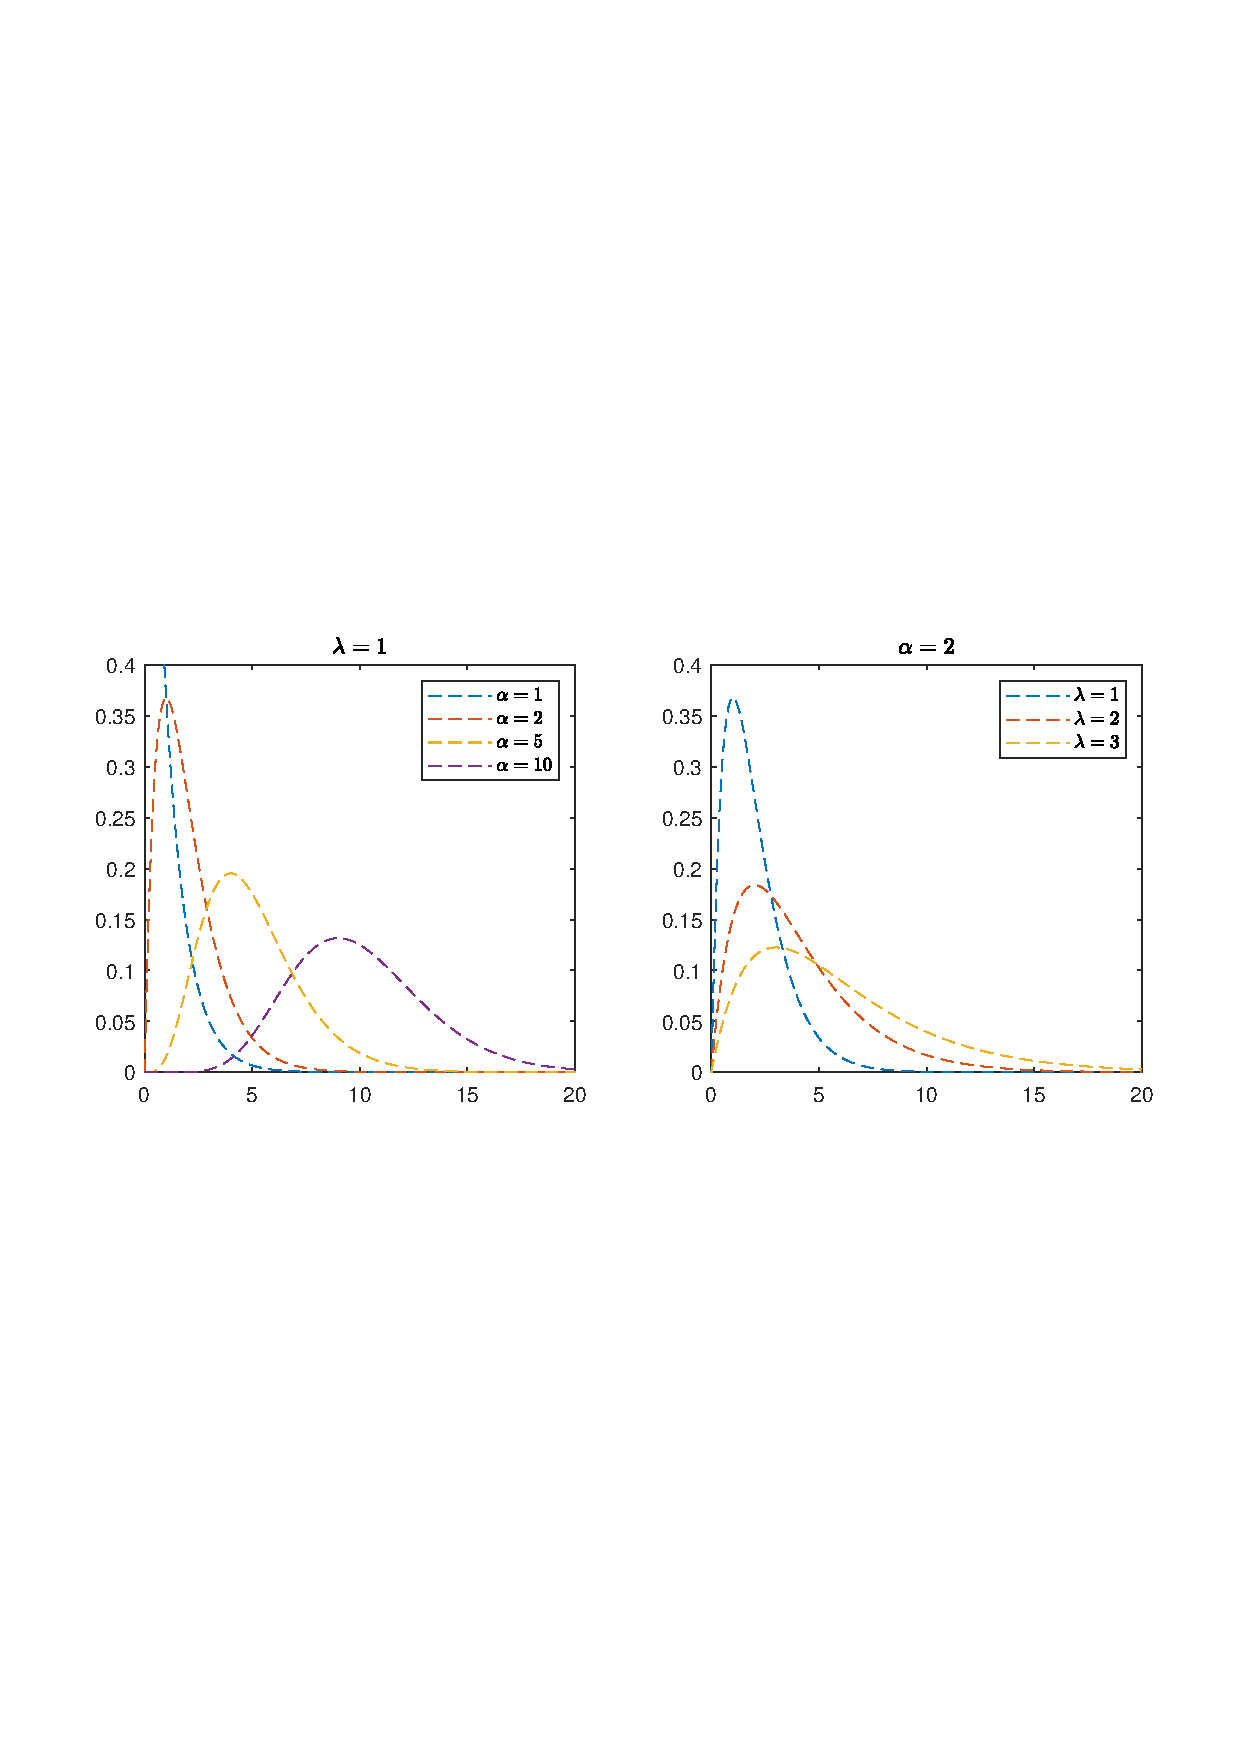
\includegraphics[width =\textwidth]{image/gamma.pdf}
    \caption{$\alpha$和$\lambda$对$Ga(\alpha, \lambda)$的影响}
    \label{fig:gamma}
\end{figure}

\begin{note}
    \begin{itemize}
        \item 由图~\ref{fig:gamma},$\alpha$影响$Ga(\alpha, \lambda)$的形状,$\lambda$影响$Ga(\alpha, \lambda)$的尺寸
        \item $\alpha\leqslant 1$时,严减;$1<\alpha\leqslant 2$时,先上凸,后下凸;$\alpha>2$时,先下凸,再上凸,最后下凸,两个拐点
        \item $\lambda$影响密度函数的胖瘦
    \end{itemize}
\end{note}

设$Z\sim Ga(\alpha, \lambda)$,则其$k$阶矩
\[
    \begin{array}{ll}
        EZ^{k}& = \displaystyle\int_{0}^{+\infty} \dfrac{\lambda^\alpha}{\Gamma(\alpha)}x^{\alpha+k-1}e^{-\lambda x}\ dx \\
        & = \dfrac{\Gamma(\alpha+k)}{\Gamma(\alpha)\lambda^k}\displaystyle\int_{0}^{+\infty} \dfrac{\lambda^{\alpha + k}}{\Gamma(\alpha+k)}x^{\alpha+k-1}e^{-\lambda x}\ dx \\
        &=\dfrac{\Gamma(\alpha+k)}{\Gamma(\alpha)\lambda^k} = \dfrac{(\alpha+k-1)(\alpha+k-2)\cdots \alpha}{\lambda^k}
    \end{array}
\]

令$\alpha = 5,\lambda = 2$,生成100个服从$Ga(5,2)$的随机数见表~\ref{tab:Ga52}。

\begin{longtable}[c]{|c|c|c|c|c|c|c|c|c|c|}
    \caption{100个服从$Ga(5,2)$的随机数}
    \label{tab:Ga52}\\
    \hline
    8.970  & 7.436  & 10.130 & 13.857 & 14.477 & 11.317 & 5.305  & 19.204 & 12.134 & 17.741 \\ \hline
    \endfirsthead
    %
    \endhead
    %
    10.786 & 15.782 & 12.751 & 7.865  & 5.020  & 7.973  & 6.702  & 11.365 & 1.864  & 8.272  \\ \hline
    6.363  & 8.856  & 11.532 & 13.531 & 12.901 & 9.747  & 3.660  & 6.329  & 11.149 & 22.713 \\ \hline
    14.703 & 1.921  & 8.829  & 12.124 & 5.686  & 22.171 & 10.194 & 6.213  & 6.221  & 11.494 \\ \hline
    8.251  & 16.907 & 8.061  & 13.385 & 2.639  & 4.600  & 12.246 & 10.625 & 8.867  & 11.413 \\ \hline
    24.037 & 6.107  & 9.044  & 20.585 & 7.057  & 6.604  & 7.033  & 9.545  & 4.226  & 3.549  \\ \hline
    6.894  & 12.698 & 10.479 & 4.221  & 8.659  & 7.955  & 3.959  & 6.650  & 14.066 & 20.703 \\ \hline
    10.081 & 2.352  & 12.030 & 13.182 & 6.721  & 11.273 & 7.286  & 4.925  & 7.724  & 12.348 \\ \hline
    8.184  & 15.014 & 6.267  & 7.876  & 8.262  & 15.584 & 26.987 & 4.301  & 11.088 & 10.851 \\ \hline
    18.763 & 15.270 & 14.215 & 9.960  & 10.059 & 11.084 & 8.172  & 14.539 & 18.870 & 6.694  \\ \hline
\end{longtable}

生成的100个随机数的经验分布函数和理论分布函数如图~\ref{fig:gammacdf}。为了与密度函数对应得比较好,我们生成5000个服从$Ga(5,2)$的随机数,如图~\ref{fig:gammapdf}。
\begin{figure}[htbp]
    \begin{minipage}[t]{0.5\textwidth}
        \centering
        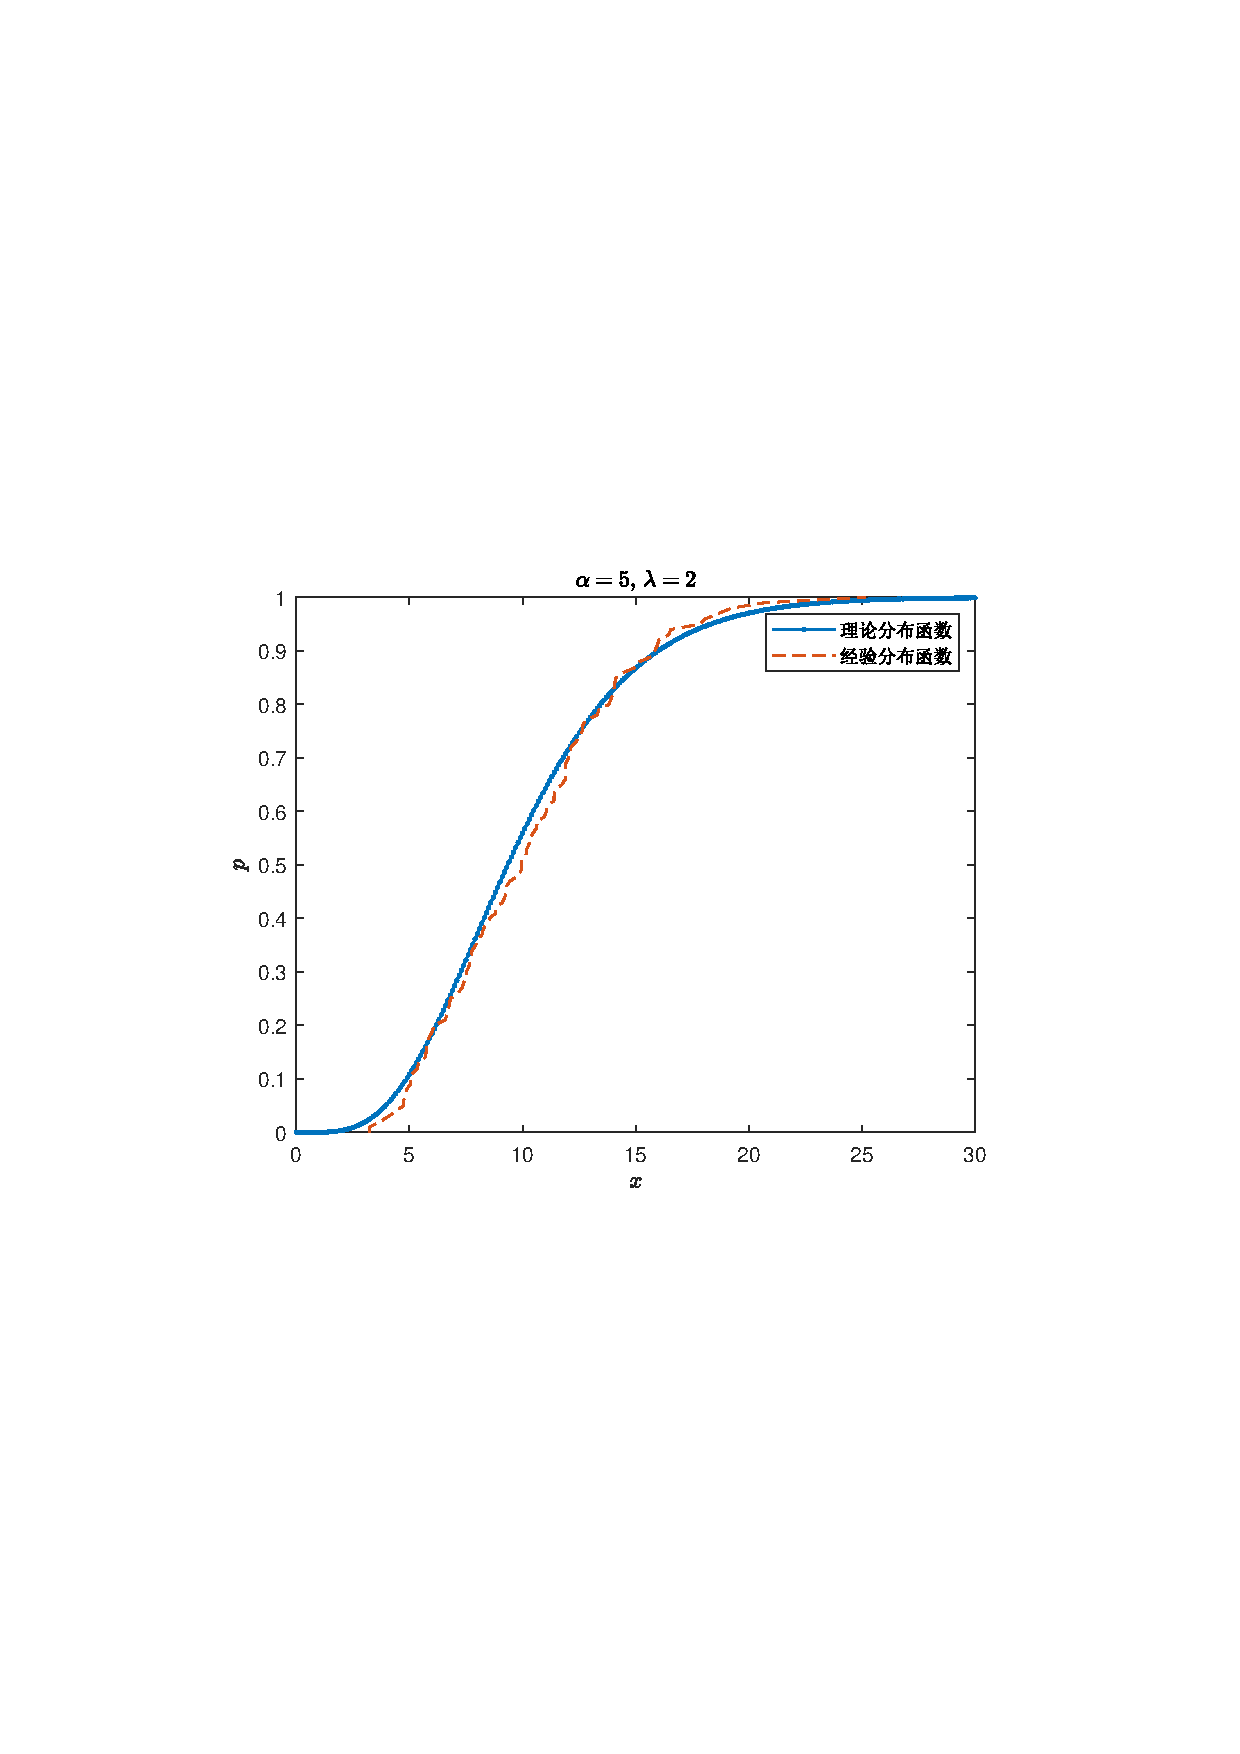
\includegraphics[width = \textwidth]{image/gammacdf.pdf}
        \caption{$Ga(5, 2)$的分布函数}
        \label{fig:gammacdf}
    \end{minipage}
    \hfill
    \begin{minipage}[t]{0.5\textwidth}
        \centering
        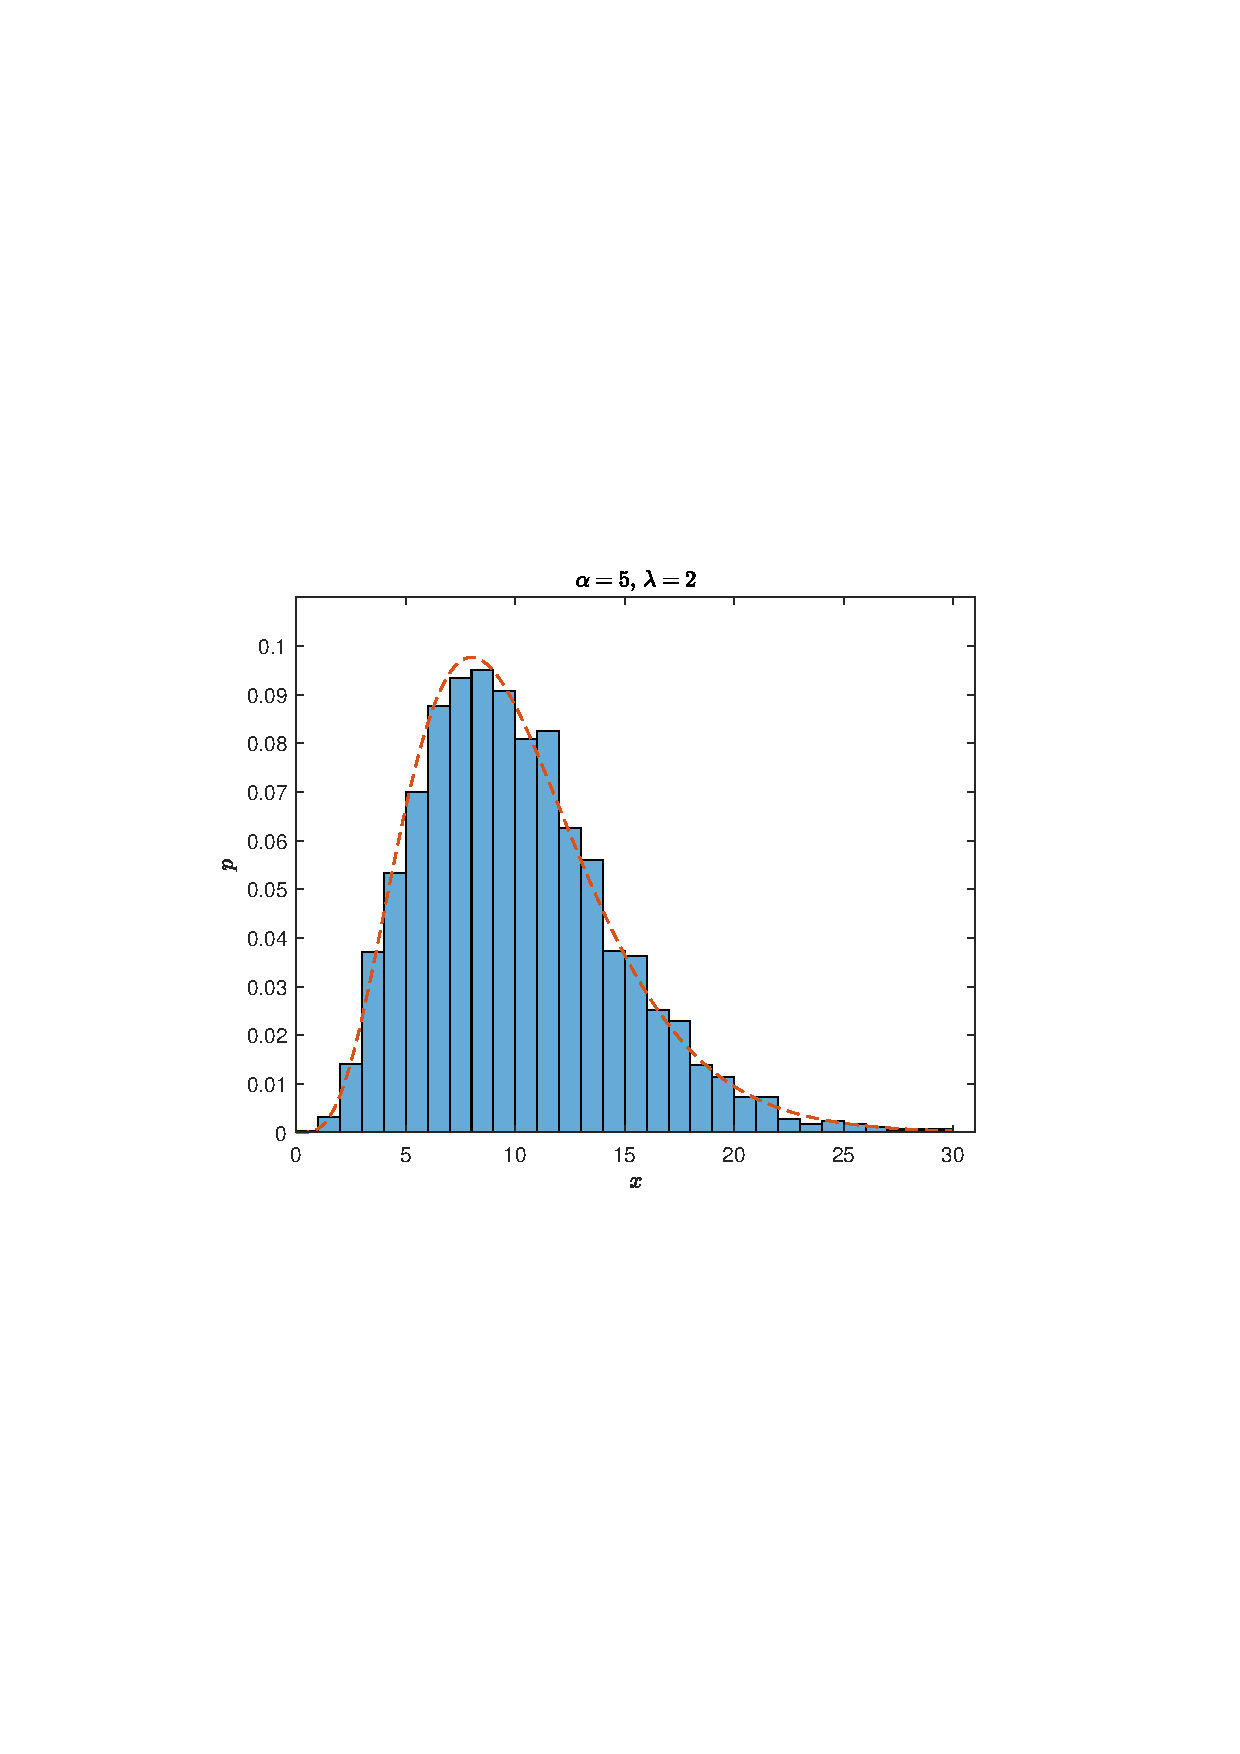
\includegraphics[width = \textwidth]{image/gammapdf.pdf}
        \caption{$Ga(5, 2)$的密度函数}
        \label{fig:gammapdf}
    \end{minipage}
\end{figure}

代码见Listing~\ref{code:gammaSamples}。
\lstinputlisting[
    style       =   matlab,
    caption     =   {\bf 生成$Ga(5, 2)$的matlab代码},
    label       =   {code:gammaSamples}
]{code/gammaSample.m}

\subsection{Beta分布族}
\begin{newdef}[Beta分布]
    设$D=(0,1)$,定义在$(D,\mathscr{B}_D)$,密度函数形如$p(x;a,b) = \dfrac{1}{B(a,b)}x^{\alpha-1}(1-x)^{b-1}I_{(0,1)}(x),\ (a>0, b>0)$的分布成为参数为$a,\ b$的Beta分布,记为$Be(a,b)$。其中$B(a,b) = \displaystyle \int_{0}^{1}x^{a-1}(1-x)^{b-1}\ dx = \dfrac{\Gamma(a)\Gamma(b)}{\Gamma(a+b)}$    
\end{newdef}

\begin{figure}[htbp]
    \centering
    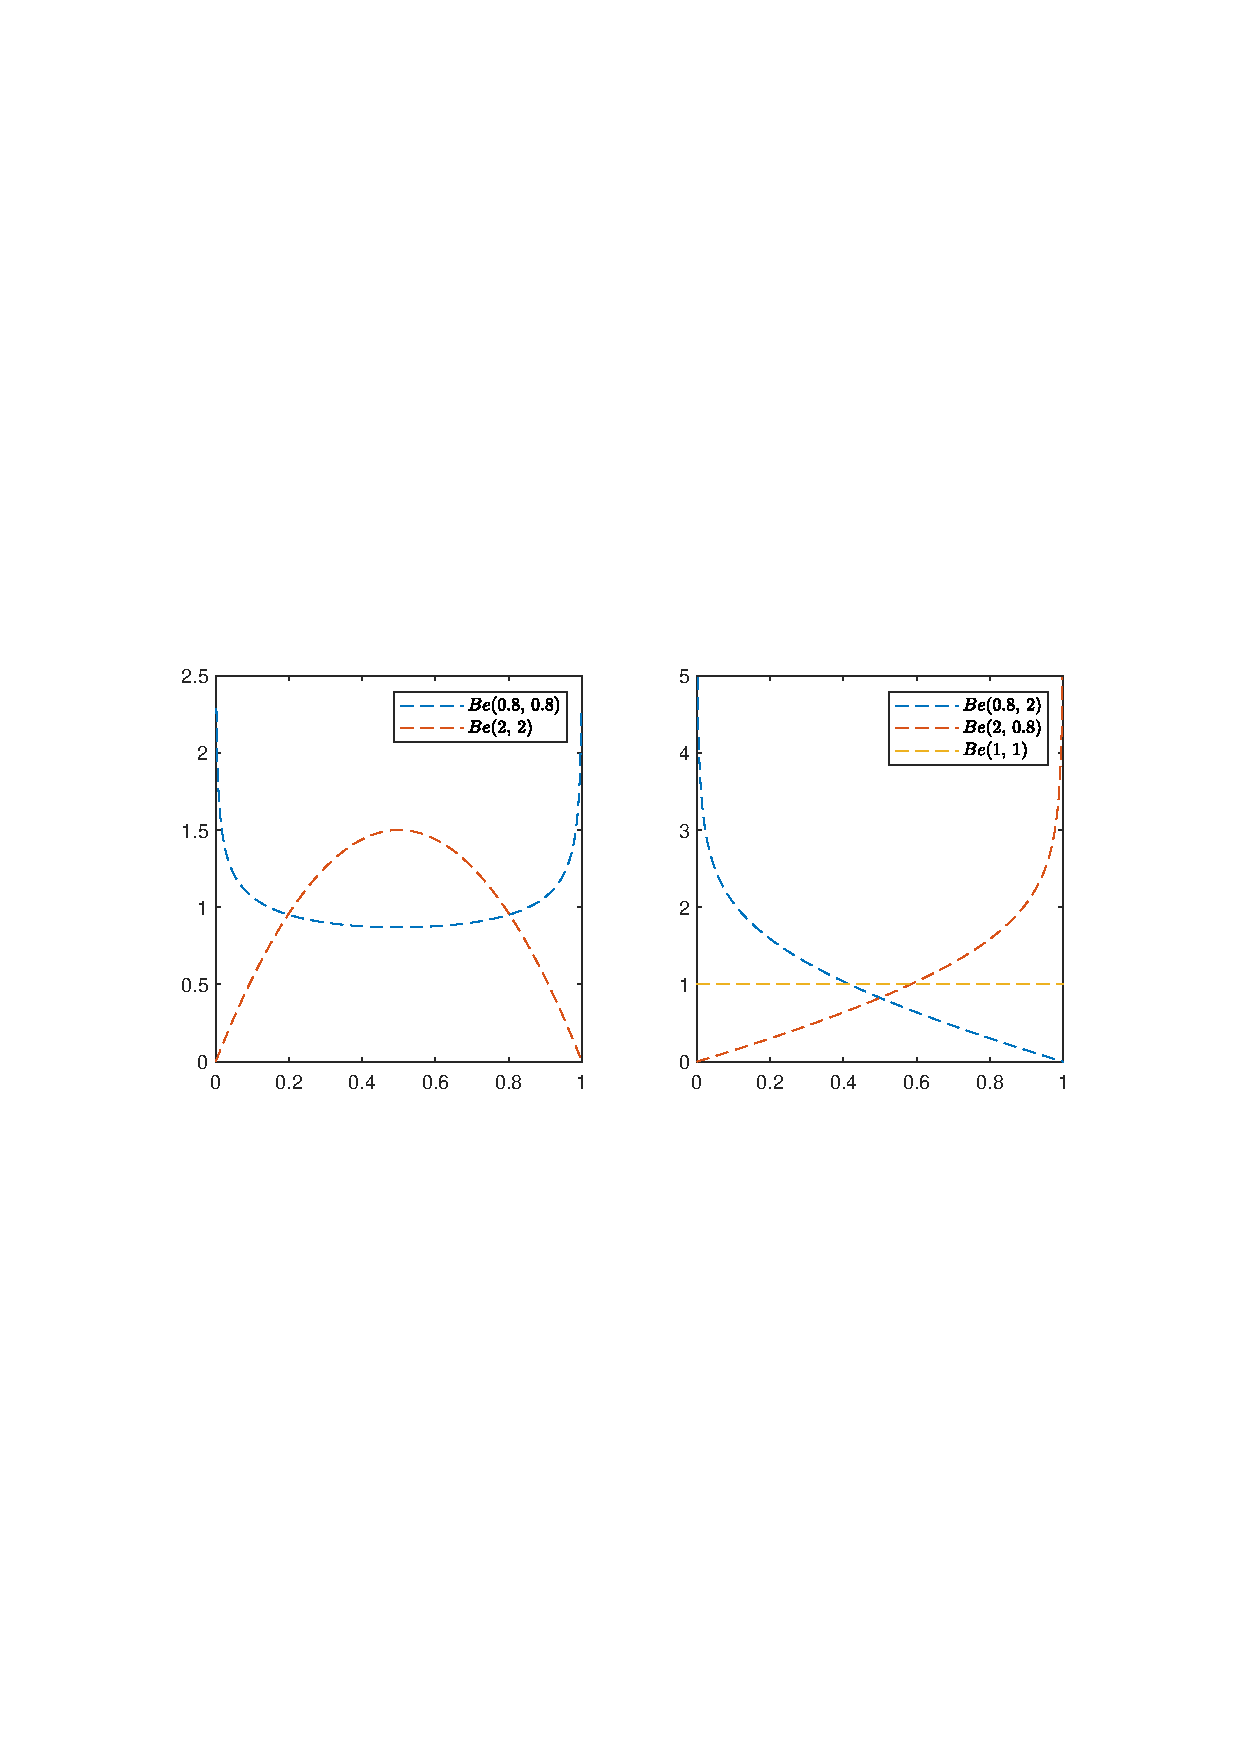
\includegraphics[width =\textwidth]{image/beta.pdf}
    \caption{$a$和$b$对$Be(a,b)$的影响}
    \label{fig:beta}
\end{figure}

\begin{note}
    由图~\ref{fig:beta}
    \begin{itemize}
        \item $a>1$和$b>1$,$p(x)$单峰状,在$x = (a-1)/(a+b-2)$处达到最大值
        \item $a<1$和$b<1$,$p(x)$U形,在$x = (a-1)/(a+b-2)$处达到最小值
        \item 当$a = b+1/2$时,Beta分布为反正弦分布
        \item $a<1$和$b>1$,$p(x)$严减
        \item $a>1$和$b<1$,$p(x)$严增
    \end{itemize}
    
\end{note}

\begin{note}
    设$Z\sim Be(a, b)$,则$Z$的$k$阶矩
    \[
        \begin{array}{ll}
            EZ^k &= \displaystyle\int_{0}^{1}\dfrac{1}{B(a,b)}x^{a+k-1}(1-x)^{b-1}\ dx\\
            &=\dfrac{B(a+k,b)}{B(a,b)}\displaystyle\int_{0}^{1}\dfrac{1}{B(a+k,1)}x^{a+k-1}(1-x)^{b-1}\ dx\\
            &= \dfrac{B(a+k,b)}{B(a,b)} = \dfrac{\Gamma(a+k)\Gamma(b)}{\Gamma(a+k+b)}\cdot \dfrac{\Gamma(a+b)}{\Gamma(a)\Gamma(b)}=\dfrac{\Gamma(a+k)\Gamma(a+b)}{\Gamma(a)\Gamma(a+k+b)}\\
            &=\dfrac{(a+k-1)(a+k-2)\cdots (a)}{(a+b+k-1)(a+b+k-2)\cdots (a+b)}
        \end{array}
    \]
    特别的,
    \[
        \begin{array}{c}
            EZ = \dfrac{a}{a+b}\\
            E^2 = \dfrac{(a+1)a}{(a+b+1)(a+b)}\\
            \operatorname{Var}Z = EZ^2-(EZ)^2=\left[ (\dfrac{a+1}{a+b+1})^2-1 \right](\dfrac{a}{a+b})^2
        \end{array}
    \]
\end{note}

令$a = 1.5,b = 2$,生成100个服从$Be(1.5,2)$的随机数见表~\ref{tab:Be1point52}

\begin{longtable}[c]{|c|c|c|c|c|c|c|c|c|c|}
    \caption{100个服从$Be(1.5,2)$的随机数}
    \label{tab:Be1point52}\\
    \hline
    0.1675 & 0.8582 & 0.9322 & 0.0391 & 0.6434 & 0.6455 & 0.2496 & 0.3051 & 0.4312 & 0.1467 \\ \hline
    \endfirsthead
    %
    \endhead
    %
    0.0999 & 0.1250 & 0.3282 & 0.2971 & 0.5698 & 0.2195 & 0.0985 & 0.5245 & 0.3720 & 0.1986 \\ \hline
    0.7823 & 0.7478 & 0.6951 & 0.5802 & 0.3194 & 0.4065 & 0.6905 & 0.1559 & 0.3785 & 0.5306 \\ \hline
    0.1999 & 0.1590 & 0.3840 & 0.3212 & 0.6368 & 0.7172 & 0.7610 & 0.3014 & 0.3848 & 0.4387 \\ \hline
    0.4263 & 0.3776 & 0.4602 & 0.3675 & 0.4937 & 0.1559 & 0.5325 & 0.3720 & 0.6380 & 0.2773 \\ \hline
    0.6846 & 0.6322 & 0.5647 & 0.1297 & 0.5743 & 0.3728 & 0.1223 & 0.6585 & 0.6322 & 0.2977 \\ \hline
    0.5291 & 0.4154 & 0.5662 & 0.0220 & 0.1352 & 0.3076 & 0.7311 & 0.7020 & 0.3809 & 0.3629 \\ \hline
    0.5882 & 0.0989 & 0.6627 & 0.0925 & 0.1623 & 0.3002 & 0.3496 & 0.3998 & 0.4126 & 0.1960 \\ \hline
    0.2560 & 0.1002 & 0.7634 & 0.5528 & 0.7717 & 0.4144 & 0.6347 & 0.3866 & 0.6521 & 0.4663 \\ \hline
    0.2750 & 0.5877 & 0.2553 & 0.6150 & 0.2477 & 0.4492 & 0.3713 & 0.1073 & 0.4405 & 0.3347 \\ \hline
\end{longtable}

生成的100个随机数的经验分布函数和理论分布函数如图~\ref{fig:betacdf},为了与密度函数对应得比较好,我们生成5000个服从$Be(1.5,2)$的随机数,绘制其分布函数,经验分布函数如图~\ref{fig:betapdf}。

\begin{figure}[htbp]
    \begin{minipage}[t]{0.5\textwidth}
        \centering
        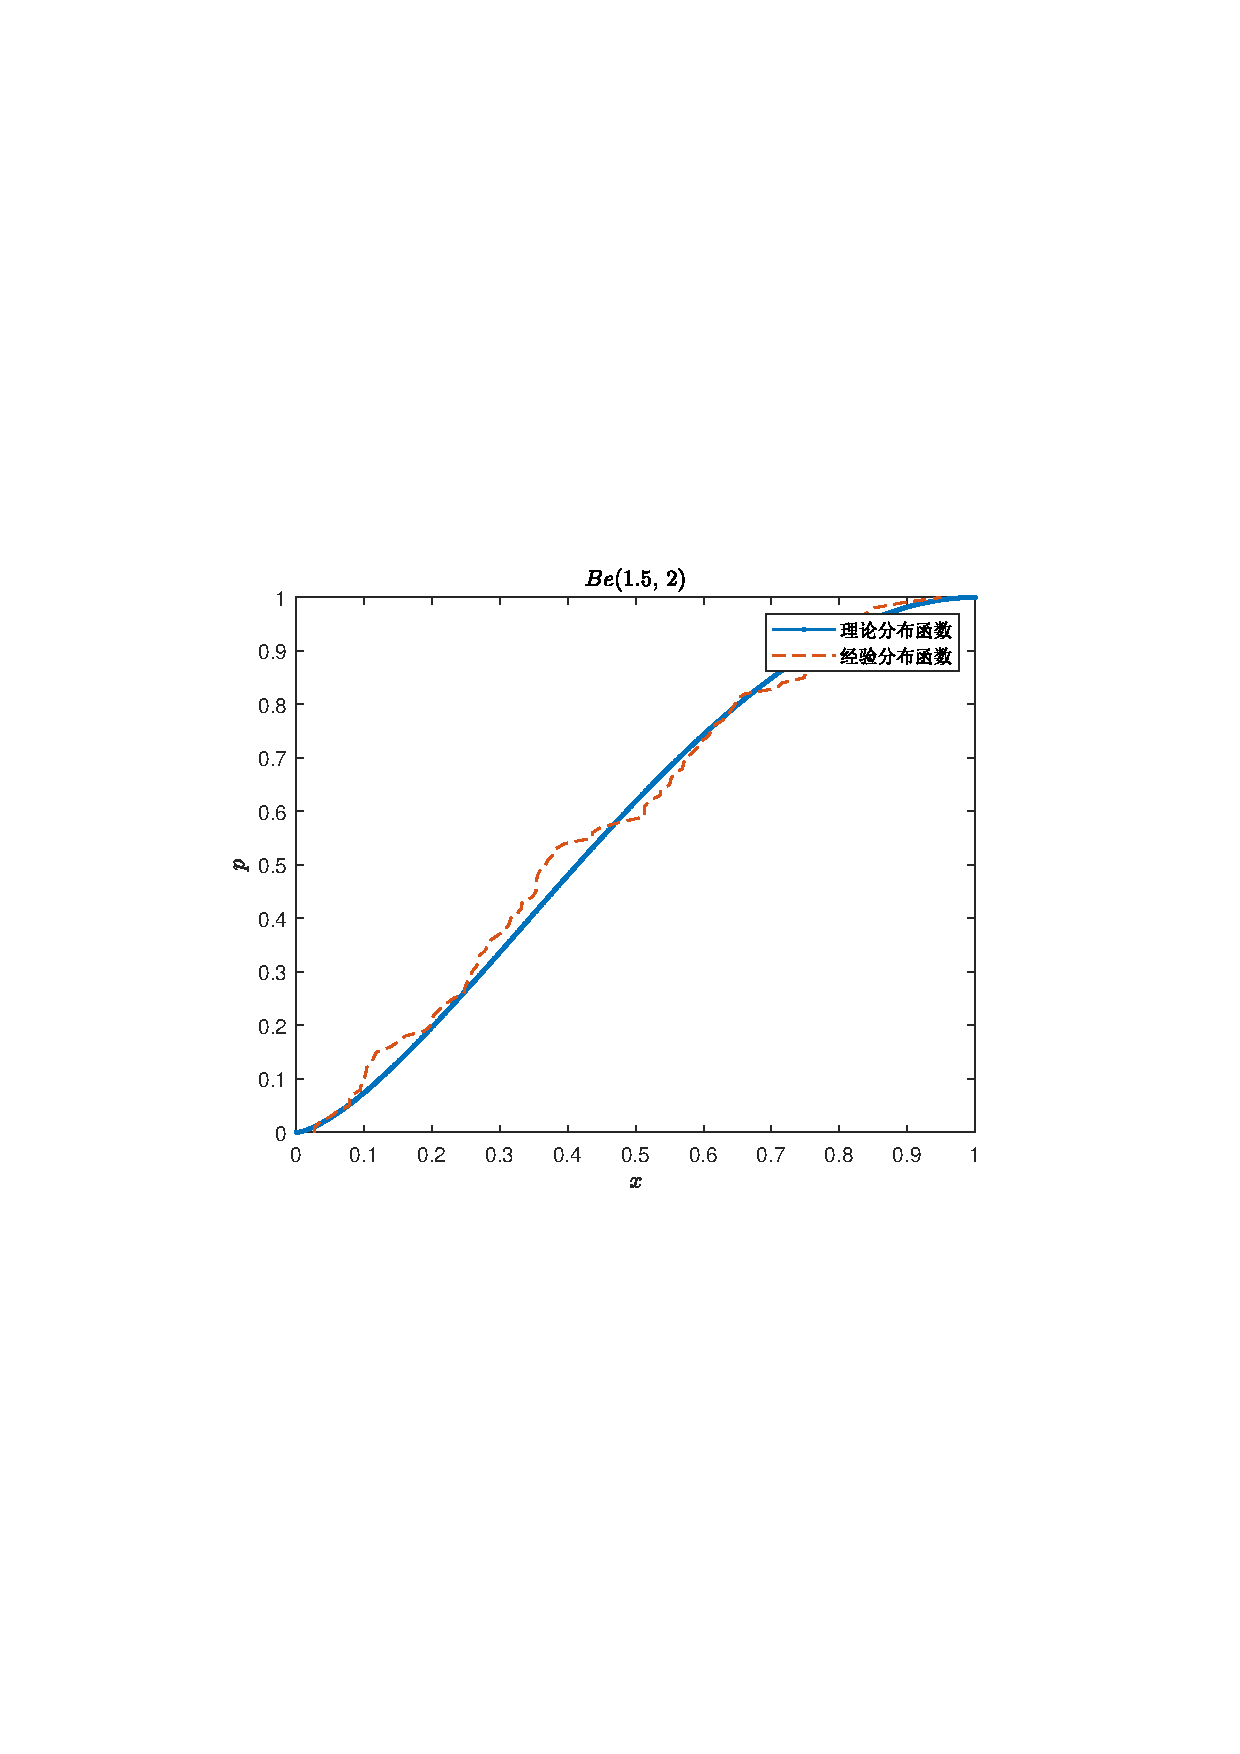
\includegraphics[width = \textwidth]{image/betacdf.pdf}
        \caption{$Be(1.5, 2)$的分布函数}
        \label{fig:betacdf}
    \end{minipage}
    \hfill
    \begin{minipage}[t]{0.5\textwidth}
        \centering
        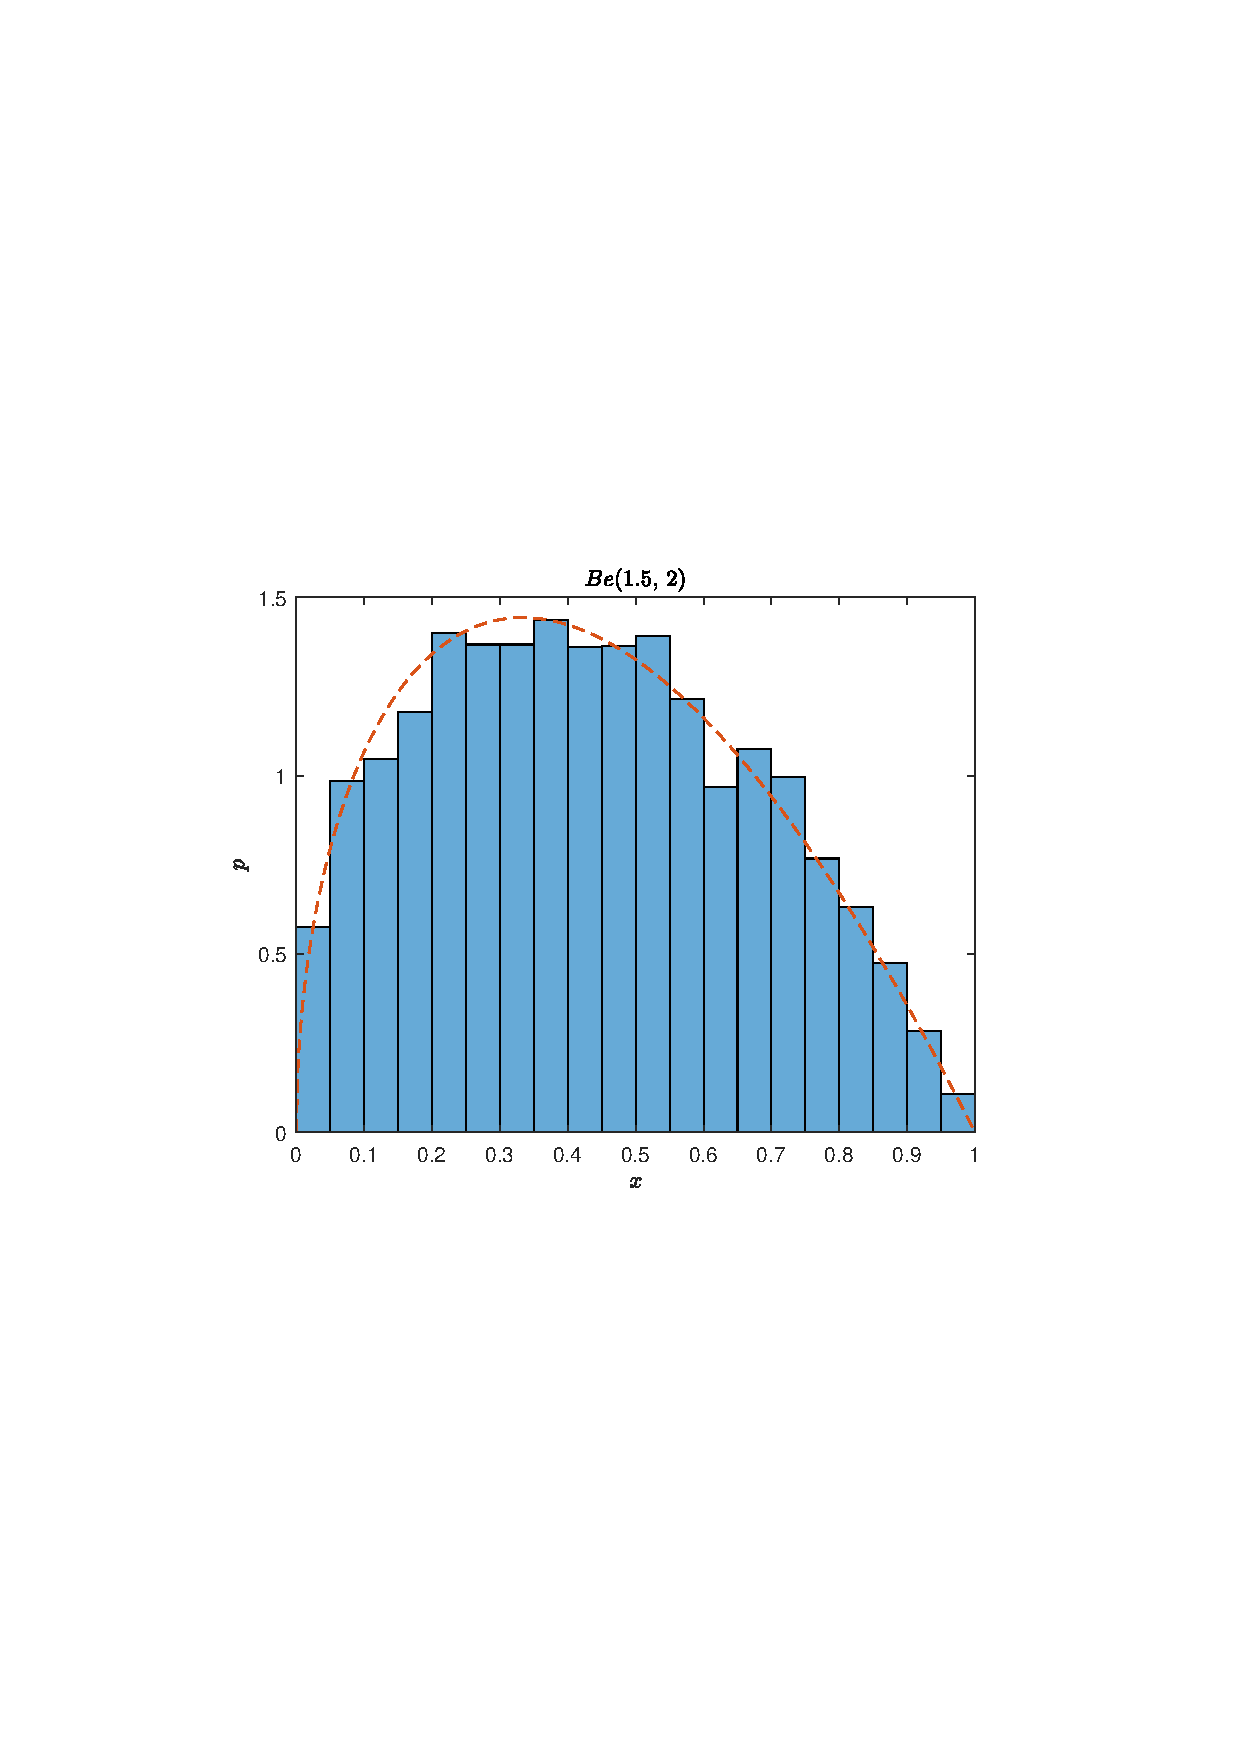
\includegraphics[width = \textwidth]{image/betapdf.pdf}
        \caption{$Be(1.5, 2)$的密度函数}
        \label{fig:betapdf}
    \end{minipage}
\end{figure}

代码见Listing~\ref{code:betaSamples}。
\lstinputlisting[
    style       =   matlab,
    caption     =   {\bf 生成$Be(1.5, 2)$的matlab代码},
    label       =   {code:betaSamples}
]{code/betaSample.m}